\documentclass[UTF8,12pt,a4paper,twoside,openright]{ctexrep}

\usepackage[a4paper,top=2.5cm,bottom=2.5cm,left=3cm,right=3cm]{geometry}
\usepackage{fontspec}
\setmainfont{Times New Roman}
\newfontfamily\tnr{Times New Roman}
\usepackage{setspace}
\usepackage{graphicx}
\usepackage{booktabs}
\usepackage{array}
\usepackage{longtable}
\usepackage{multirow}
\usepackage{amsmath,amssymb}
\usepackage[labelsep=space]{caption}
\usepackage{subcaption}
\usepackage{float}
\usepackage{indentfirst}
\usepackage{hyperref}
\usepackage{fancyhdr}
\usepackage{titlesec}
\usepackage{tocloft}
\usepackage{lastpage}
\usepackage[backend=biber,style=gb7714-2015]{biblatex}

\addbibresource{bib/references.bib}

\hypersetup{
    colorlinks=true,
    linkcolor=black,
    citecolor=black,
    urlcolor=black
}

\setlength{\parindent}{2em}
\setlength{\parskip}{0pt}
\setlength{\headheight}{14.5pt}
\setcounter{secnumdepth}{3}
\setcounter{tocdepth}{2}

\newcommand{\thesisheadertext}{成都信息工程大学学士学位论文}
\newcommand{\thesisbodyfont}{\songti\fontsize{12pt}{20pt}\selectfont}
\newcommand{\thesiswuhao}{\songti\fontsize{10.5pt}{15pt}\selectfont}
\newcommand{\thesissmallfive}{\songti\fontsize{9pt}{11pt}\selectfont}
\newcommand{\thesispageline}{%
    {\thesissmallfive 第{\tnr\thepage}页\quad 共{\tnr\pageref{LastPage}}页}%
}
\newcommand{\thesisfrontpage}{%
    {\tnr\fontsize{9pt}{11pt}\selectfont\thepage}%
}

\AtBeginDocument{\thesisbodyfont}
\linespread{1.0}\selectfont

\DeclareCaptionFont{thesiscaptionfont}{\songti\fontsize{10.5pt}{15pt}\selectfont}
\captionsetup{
    font=thesiscaptionfont,
    labelfont=normalfont,
    textfont=normalfont,
    justification=centering,
    singlelinecheck=false
}
\captionsetup*[figure]{position=bottom,skip=6pt}
\captionsetup*[table]{position=top,skip=6pt}
\renewcommand{\figurename}{图}
\renewcommand{\tablename}{表}

\numberwithin{figure}{chapter}
\numberwithin{table}{chapter}
\numberwithin{equation}{chapter}
\renewcommand{\thefigure}{\arabic{chapter}-\arabic{figure}}
\renewcommand{\thetable}{\arabic{chapter}-\arabic{table}}
\renewcommand{\theequation}{\arabic{chapter}-\arabic{equation}}

\titleformat{\chapter}
    {\centering\songti\bfseries\fontsize{16pt}{20pt}\selectfont}
    {第\arabic{chapter}章}
    {1em}
    {}
\titleformat{\section}
    {\songti\bfseries\fontsize{14pt}{20pt}\selectfont}
    {\thesection}
    {1em}
    {}
\titleformat{\subsection}
    {\songti\bfseries\fontsize{12pt}{20pt}\selectfont}
    {\thesubsection}
    {1em}
    {}
\titleformat{\subsubsection}
    {\songti\fontsize{12pt}{20pt}\selectfont}
    {\thesubsubsection}
    {1em}
    {}

\titlespacing*{\chapter}{0pt}{0pt}{20pt}
\titlespacing*{\section}{0pt}{12pt}{6pt}
\titlespacing*{\subsection}{0pt}{12pt}{6pt}
\titlespacing*{\subsubsection}{0pt}{6pt}{6pt}

\renewcommand{\contentsname}{目\quad 录}
\renewcommand{\cfttoctitlefont}{\hfill\songti\bfseries\fontsize{16pt}{20pt}\selectfont}
\renewcommand{\cftaftertoctitle}{\hfill}
\renewcommand{\cftchapfont}{\songti\fontsize{12pt}{20pt}\selectfont}
\renewcommand{\cftsecfont}{\songti\fontsize{12pt}{20pt}\selectfont}
\renewcommand{\cftsubsecfont}{\songti\fontsize{12pt}{20pt}\selectfont}
\renewcommand{\cftchappagefont}{\tnr\fontsize{12pt}{20pt}\selectfont}
\renewcommand{\cftsecpagefont}{\tnr\fontsize{12pt}{20pt}\selectfont}
\renewcommand{\cftsubsecpagefont}{\tnr\fontsize{12pt}{20pt}\selectfont}
\renewcommand{\cftdotsep}{1}
\cftsetindents{chapter}{0em}{5em}
\cftsetindents{section}{2em}{4em}
\cftsetindents{subsection}{4em}{5em}
\setlength{\cftbeforechapskip}{0pt}
\setlength{\cftbeforesecskip}{0pt}
\setlength{\cftbeforesubsecskip}{0pt}

\makeatletter
\newcommand{\customtableofcontents}{
    \chapter*{\contentsname}
    \markboth{\thesisheadertext}{\thesisheadertext}
    \noindent\hfill{\songti\fontsize{12pt}{20pt}\selectfont 论文总页数：{\tnr\pageref{LastPage}}页}\par
    \vspace{0.5em}
    \@starttoc{toc}
}
\makeatother

\fancypagestyle{thesis-decl}{
    \fancyhf{}
    \fancyhead[C]{{\songti\fontsize{9pt}{11pt}\selectfont \thesisheadertext}}
    \renewcommand{\headrulewidth}{0.4pt}
    \renewcommand{\footrulewidth}{0pt}
}

\fancypagestyle{thesis-front}{
    \fancyhf{}
    \fancyhead[C]{{\songti\fontsize{9pt}{11pt}\selectfont \thesisheadertext}}
    \fancyfoot[C]{\thesisfrontpage}
    \renewcommand{\headrulewidth}{0.4pt}
    \renewcommand{\footrulewidth}{0pt}
}

\fancypagestyle{thesis-main}{
    \fancyhf{}
    \fancyhead[C]{{\songti\fontsize{9pt}{11pt}\selectfont \thesisheadertext}}
    \fancyfoot[C]{\thesispageline}
    \renewcommand{\headrulewidth}{0.4pt}
    \renewcommand{\footrulewidth}{0pt}
}

\defbibheading{bibintoc}[\bibname]{%
    \chapter*{#1}
    \addcontentsline{toc}{chapter}{#1}
    \markboth{\thesisheadertext}{\thesisheadertext}
}
\renewcommand*{\bibfont}{\songti\fontsize{10.5pt}{20pt}\selectfont}

\begin{document}

\pagestyle{empty}
\begin{titlepage}
\thispagestyle{empty}

\begin{center}
{\songti\bfseries\fontsize{12pt}{20pt}\selectfont 中图分类号：{\tnr\bfseries TP391.41} \hspace{2.2cm} 学校代码：{\tnr\bfseries 10621}}

\vspace{0.6cm}

{\songti\bfseries\fontsize{12pt}{20pt}\selectfont {\tnr\bfseries UDC}分类号：{\tnr\bfseries 004.932:616-073.756.8} \hspace{1.2cm} 密级：公开}

\vspace{1.2cm}

{\heiti\bfseries\zihao{2} 成都信息工程大学}

\vspace{0.6cm}

{\heiti\bfseries\zihao{2} 学士学位论文}

\vspace{1.4cm}

{\songti\bfseries\fontsize{16pt}{20pt}\selectfont
\parbox{0.94\textwidth}{\centering 基于{\tnr\bfseries 3DGS}与{\tnr\bfseries StyleGAN2}的{\tnr\bfseries MRI}医学图像拟生成平台的设计与实现}}

\vspace{0.5cm}

{\tnr\bfseries\fontsize{16pt}{20pt}\selectfont
\parbox{0.92\textwidth}{\centering Design and Implementation of an MRI Medical Image Pseudo-Generation Platform Based on 3DGS and StyleGAN2}}

\vspace{1.2cm}
\end{center}

\renewcommand{\arraystretch}{1.55}
\newcommand{\coverlabel}[1]{{\fangsong\fontsize{14pt}{20pt}\selectfont\makebox[3.6cm][s]{#1}}}
\newcommand{\coverfield}[1]{\underline{\makebox[8.2cm][c]{#1}}}
\begin{center}
\begin{tabular}{p{3.6cm} p{8.2cm}}
\coverlabel{姓\hfill 名} & \coverfield{{\fangsong\fontsize{14pt}{20pt}\selectfont 黎曜玮}} \\
\coverlabel{学\hfill 号} & \coverfield{{\tnr\bfseries\fontsize{14pt}{20pt}\selectfont 2022132078}} \\
\coverlabel{学\hfill 院} & \coverfield{{\fangsong\fontsize{14pt}{20pt}\selectfont 人工智能学院}} \\
\coverlabel{专\hfill 业} & \coverfield{{\fangsong\fontsize{14pt}{20pt}\selectfont 人工智能}} \\
\coverlabel{研\hfill 究\hfill 方\hfill 向} & \coverfield{{\fangsong\fontsize{14pt}{20pt}\selectfont 医学图像智能处理}} \\
\coverlabel{指\hfill 导\hfill 教\hfill 师} & \coverfield{{\fangsong\fontsize{14pt}{20pt}\selectfont 何长春\quad 讲师}} \\
\coverlabel{辅助指导教师} & \coverfield{{\fangsong\fontsize{14pt}{20pt}\selectfont 无}} \\
\coverlabel{论文提交日期} & \coverfield{{\tnr\bfseries\fontsize{14pt}{20pt}\selectfont 2026}{\fangsong\fontsize{14pt}{20pt}\selectfont \hspace{1em}年\hspace{1em}}{\tnr\bfseries\fontsize{14pt}{20pt}\selectfont 5}{\fangsong\fontsize{14pt}{20pt}\selectfont \hspace{1em}月}} \\
\end{tabular}
\end{center}

\end{titlepage}

\cleardoublepage

\pagestyle{thesis-decl}
\chapter*{\texorpdfstring{{\songti\bfseries\fontsize{16pt}{20pt}\selectfont 成都信息工程大学\\[0.5em]学士学位论文原创性声明}}{原创性声明}}
\thispagestyle{thesis-decl}
\markboth{成都信息工程大学学士学位论文}{成都信息工程大学学士学位论文}

{\songti\fontsize{12pt}{20pt}\selectfont
本人郑重声明：所呈交的学位论文《基于 StyleGAN2 与 3DGS 的 MRI 医学图像生成平台的设计与实现》，是本人在指导教师指导下进行研究工作所取得的成果。除文中已经注明引用的内容外，本学位论文的研究成果不包含任何他人创作的、已公开发表或者没有公开发表的作品内容。对本论文所涉及研究工作做出贡献的其他个人和集体，均已在文中以明确方式标明。本学位论文原创性声明的法律责任由本人承担。
\par}

\vspace{3cm}

\noindent{\songti\fontsize{12pt}{20pt}\selectfont 论文作者签名：}\hspace{4cm}{\songti\fontsize{12pt}{20pt}\selectfont 年\hspace{1cm}月\hspace{1cm}日}

\vspace{2cm}

\noindent{\songti\fontsize{12pt}{20pt}\selectfont 指导教师签名：}\hspace{4cm}{\songti\fontsize{12pt}{20pt}\selectfont 年\hspace{1cm}月\hspace{1cm}日}

\cleardoublepage

\thesisdecltitle{成都信息工程大学}{学士学位论文版权使用授权书}

\vspace{0.4em}

\begin{thesisdeclbody}
本人完全了解成都信息工程大学关于收集、保存、使用学位论文的规定，同意如下各项内容：按照学校要求提交学位论文的印刷本和电子版本；学校有权保存学位论文的印刷本和电子版，并采用影印、缩印、扫描、数字化或其它手段保存论文；学校有权提供目录检索以及提供本学位论文全文或者部分的阅览服务；学校有权按有关规定向国家有关部门或者机构送交论文的复印件和电子版；学校可以复制、赠送和交换学位论文；学校可以公布学位论文的全部或部分内容。（保密学位论文在解密后遵守此规定）

除非另有科研合同和其他法律文书的制约，本论文的科研成果属于成都信息工程大学。
\end{thesisdeclbody}

\vspace{0.2em}

\thesisdeclsignline{论文作者签名：}

{\thesisdeclbodyfont\noindent\hspace*{2em}本学位论文密级属于\hspace{1.2cm}级，保密期限为\hspace{1.2cm}年，解密后适用本授权书。\par}

\vspace{0.4em}

\begin{center}
{\thesisdeclbodyfont
\renewcommand{\arraystretch}{1.45}
\begin{tabular}{|>{\centering\arraybackslash}p{2.3cm}|>{\centering\arraybackslash}p{2.5cm}|>{\centering\arraybackslash}p{2.3cm}|>{\centering\arraybackslash}p{3.7cm}|}
\hline
密\hspace{1em}级 &  & 解密时间 & 年\hspace{1.1cm}月\hspace{1.1cm}日 \\
\hline
学位论文作者签名 & 年\hspace{0.4cm}月\hspace{0.4cm}日 & 指导教师签名 & 年\hspace{0.8cm}月\hspace{0.8cm}日 \\
\hline
\multicolumn{2}{|c|}{学校保密办公室审核情况} & \multicolumn{2}{c|}{年\hspace{1.1cm}月\hspace{1.1cm}日（公章）} \\
\hline
\end{tabular}
}
\end{center}

\vspace{0.2em}

\thesisdeclnote{注：答辩通过后，最终版论文中，均须附由作者本人签名的原创声明及使用授权书。}

\cleardoublepage

\pagenumbering{roman}
\pagestyle{thesis-front}
\chapter*{\texorpdfstring{{\songti\bfseries\fontsize{16pt}{20pt}\selectfont 摘\quad 要}}{摘要}}
\thispagestyle{thesis-front}
\markboth{成都信息工程大学学士学位论文}{成都信息工程大学学士学位论文}

{\songti\fontsize{12pt}{20pt}\selectfont
真实 MRI 数据受采集成本、隐私保护和伦理审查等因素限制，单张二维切片也难以完整呈现脑部结构的空间关系。基于这一现实问题，本文设计并实现了一套基于 3DGS 与 StyleGAN2 的 MRI 医学图像拟生成平台。平台将 NIfTI 数据预处理、二维切片生成、连续序列组织、点云初始化、3DGS 训练与重建和交互展示串联为一条相对完整的实验链路。实验以 IXI 脑部 MRI 数据为基础，完成体数据切片、灰度归一化、分辨率统一、低信息切片过滤和 StyleGAN2-ADA 训练集构建，并训练得到可接入平台推理的二维 MRI 切片生成模型。三维部分选取 180 张连续 MRI 切片作为监督图像，以 300000 点初始点云作为空间起点，经过 30000 轮 3DGS 训练后得到包含 556424 个高斯点的三维表达结果，并导出 60000 点预览点云用于前端交互展示。工程实现采用 FastAPI + React 架构，后端提供数据、生成、分析、任务和三维资产接口，前端承担仪表盘、生成工作台、医学影像查看器、影像分析报告、可信性评估、点云展示和 AI 助手等交互功能。实验结果显示，训练后的 StyleGAN2 权重能够生成具有脑部 MRI 灰度轮廓的二维切片；3DGS 在第 30000 轮训练时达到 L1 为 0.0459、PSNR 为 20.0909 dB。结合训练日志、模型权重、渲染切片、指标曲线和前端展示资产可以看出，平台已经形成从 MRI 数据整理到二维生成、再到三维高斯表达的可复现实验流程。
\par}

\vspace{1em}

\noindent{\songti\bfseries\fontsize{12pt}{20pt}\selectfont 关键词}{\songti\fontsize{12pt}{20pt}\selectfont ：MRI 医学图像；3D Gaussian Splatting；StyleGAN2；医学图像拟生成；教学平台}

\cleardoublepage

\chapter*{\texorpdfstring{{\tnr\bfseries\fontsize{14pt}{20pt}\selectfont ABSTRACT}}{ABSTRACT}}
\thispagestyle{thesis-front}
\markboth{成都信息工程大学学士学位论文}{成都信息工程大学学士学位论文}

\begin{thesisenabstract}
Real magnetic resonance imaging (MRI) data is difficult to use directly in teaching demonstrations and generative model experiments because of acquisition cost, privacy protection, and ethical review. A single two-dimensional slice also gives only limited insight into the spatial structure of the brain. Based on this practical need, this thesis designs and implements an MRI medical image pseudo-generation platform built on 3D Gaussian Splatting (3DGS) and StyleGAN2. The IXI brain MRI dataset is used as the data source. The preprocessing stage includes Neuroimaging Informatics Technology Initiative (NIfTI) volume slicing, intensity normalization, resolution standardization, low-information slice filtering, and StyleGAN2-ADA dataset construction. A two-dimensional MRI slice generator is then trained and connected to the platform for inference. In the three-dimensional stage, 180 continuous MRI slices are used as supervision, and a 300000-point initial point cloud serves as the spatial starting point. After 30000 iterations of 3DGS training, the system obtains a representation with 556424 Gaussian points, and a 60000-point preview cloud is exported for frontend interaction. The engineering platform uses a FastAPI and React architecture. The backend manages data, generation, analysis, task, and 3D asset APIs, while the frontend provides the dashboard, generation workbench, medical image viewer, image analysis report, trust evaluation, point cloud display, and AI assistant. Experimental records show that the trained StyleGAN2 model can generate MRI-like slices with recognizable brain grayscale structures. At iteration 30000, 3DGS training reaches an L1 loss of 0.0459 and a PSNR of 20.0909 dB. These metrics mainly reflect rendering reconstruction consistency in this experiment. Project logs, model snapshots, rendered slices, metric curves, and frontend display assets together show that the platform provides a reproducible workflow from MRI data processing to two-dimensional generation and three-dimensional Gaussian representation.
\end{thesisenabstract}

\begin{thesisenkeywords}
\noindent{\bfseries Key Words}{: MRI Medical Image; 3D Gaussian Splatting; StyleGAN2; Medical Image Pseudo-Generation; Teaching Platform}
\end{thesisenkeywords}

\cleardoublepage

\customtableofcontents
\cleardoublepage

\pagenumbering{arabic}
\pagestyle{thesis-main}
\chapter{绪论}

\section{课题背景}
医学影像记录人体结构和病理变化，是临床诊断、疾病筛查、治疗规划和医学教学中经常使用的资料。磁共振成像（Magnetic Resonance Imaging，MRI）具有较好的软组织对比度，不使用电离辐射，也支持多序列成像。正因为这些特点，MRI 在脑部结构观察、神经系统疾病分析和医学影像教学中具有较高使用价值。

在实际教学和模型实验中，真实 MRI 数据并不总是容易获取和使用。扫描设备成本较高，病例数据又涉及隐私保护和伦理审查，数据标注也常常需要医学专业知识参与。即使能够获得公开数据，不同设备和扫描协议仍会带来灰度分布差异。对人工智能模型来说，数据规模和数据一致性都会影响训练稳定性；对课堂演示和毕业设计展示来说，仅给出单张二维切片，也很难把三维结构关系讲清楚。

生成式人工智能为医学影像教学和实验提供了新的思路。生成对抗网络（Generative Adversarial Network，GAN）通过生成器和判别器的对抗训练学习数据分布，已被用于图像生成、图像增强和跨模态合成等任务\cite{goodfellow2014gan,skandarani2023gans,khader2023ddpm3d}。StyleGAN 系列模型重视图像质量和潜空间控制。StyleGAN2 改进了生成器结构和正则化方式，生成图像质量也进一步提高\cite{karras2020stylegan2}。StyleGAN2-ADA 通过自适应数据增强缓解有限数据训练中的过拟合问题\cite{karras2020ada}。本文选择这一框架，主要是考虑到 MRI 切片灰度结构相对集中，且训练数据来源有限。

当二维切片可以生成之后，新的问题随之出现：这些切片如何被组织成更容易理解的空间表达。三维高斯泼溅（3D Gaussian Splatting，3DGS）使用可优化的三维高斯基元表示场景，并通过可微渲染生成视图\cite{kerbl20233dgs}。原始 3DGS 主要面向多视角照片重建，而 MRI 切片与普通照片的成像方式并不相同。因此，本课题没有简单套用自然场景重建流程，而是借鉴点云初始化和三维高斯表达思路，将连续 MRI 切片组织起来，并通过平台展示三维结果。由此形成了“二维生成 + 三维表达 + 平台展示”的研究路线。

\section{国内外研究现状}
医学图像生成研究主要服务于数据扩充、隐私保护、跨模态合成和辅助教学。早期方法常通过旋转、缩放、裁剪和灰度扰动来扩充数据。这类方法实现简单，但本质上仍是在改变已有图像，难以产生新的结构变化。深度生成模型出现后，GAN、变分自编码器和扩散模型逐渐被用于医学图像合成。

近年医学图像生成研究更加关注数据稀缺、隐私保护和下游任务可用性。Skandarani 等在多模态医学图像合成实验中指出，不同 GAN 架构在 MRI、CT 和眼底图像上的表现并不一致，视觉真实并不必然带来下游任务提升\cite{skandarani2023gans}。Khader 等研究了扩散模型在三维医学图像生成中的应用，说明高质量合成数据需要同时关注图像外观、解剖合理性和切片一致性\cite{khader2023ddpm3d}。Müller-Franzes 等进一步比较了潜在扩散模型与 GAN 在医学图像合成中的表现，提示生成模型评价不能只依赖单一视觉指标\cite{mullerfranzes2023comparison}。Akbar 等围绕脑肿瘤 MR 合成图像开展分割实验，也强调合成数据需要通过具体任务验证其实际价值\cite{akbar2024syntheticmr}。基于这些研究，本文把平台用途限定为教学演示和工程验证，不把输出结果用于临床诊断。

GAN 方法的发展为本课题提供了二维生成基础。Goodfellow 等提出的 GAN 建立了对抗式生成学习的基本框架\cite{goodfellow2014gan}。StyleGAN 引入基于风格的生成结构和中间潜空间，提高了图像合成质量\cite{karras2019stylegan}。StyleGAN2 在此基础上改进结构，并减少原 StyleGAN 中的伪影问题\cite{karras2020stylegan2}。StyleGAN2-ADA 面向有限数据训练场景，使用自适应数据增强提升训练稳定性\cite{karras2020ada}。在更近的脑影像生成研究中，Tudosiu 等强调了三维脑影像生成对形态保持和结构合理性的要求\cite{tudosiu2024brain}。本课题使用公开 MRI 数据切片，病例来源和结构类型仍有限，因此选用 StyleGAN2-ADA 作为二维 MRI 切片生成框架，并在论文中明确其教学演示边界。

三维展示部分更强调工程适配。传统医学三维展示常使用体绘制、表面重建或体素显示，这些方法适合展示真实体数据。本文的输入还包括生成切片，所以必须处理切片连续性、坐标尺度和灰度一致性。3DGS 从点云出发，并用三维高斯表示空间结构\cite{kerbl20233dgs}。2024 年以来，已有研究把 3DGS 引入内窥镜重建、手术场景重建和合成数据生成等医学相关任务，说明显式高斯表示在医学视觉场景中具有较好的工程拓展性\cite{bonilla2024gaussianpancakes,huang2024endo4dgs,guo2024freesurgs,zeng2024surgical3dgs}。因此，本课题把重点放在工程链路上：完成二维切片到点云的转换，并把点云和连续切片用于 3DGS 训练与展示。

\section{项目研究意义}
本课题的价值不只在于复现某一个模型，更在于把原本分散的实验步骤整理成一个可以运行和展示的平台流程。MRI 数据读取、切片预处理、StyleGAN2 训练、图像生成、点云构建、3DGS 训练和结果展示被放在同一条链路中，脚本输出不再只是零散文件，而可以通过页面、日志和图像结果进行查看。

从医学图像智能处理角度看，本课题探索了 StyleGAN2-ADA 在脑部 MRI 二维切片生成中的使用方式，并把生成切片继续组织为连续序列和三维点云。这样处理后，二维生成结果不再停留在单张图片层面，而可以进入后续三维表达流程。对学习者而言，这种设计更容易说明医学体数据从切片到空间结构的转换过程。

从教学应用角度看，平台采用 FastAPI + React 构建前后端分离界面。用户不需要反复输入复杂命令，就可以在网页中完成数据查看、模型生成、影像分析、任务追踪和三维结果展示。这样的形式更适合人工智能专业医学图像处理方向的课程演示、实验复核和毕业答辩展示。

\section{论文主要内容与章节安排}
围绕上述目标，论文工作主要包括四个部分。

第一部分是 MRI 数据预处理。系统读取 IXI 数据集中 NIfTI 格式的 T1 脑部 MRI 数据，提取轴向切片，并完成百分位归一化、尺寸统一和低信息切片过滤。处理后的数据可用于 StyleGAN2-ADA 训练。

第二部分是二维 MRI 切片生成。系统基于预处理切片训练 StyleGAN2-ADA，并在平台中支持权重加载、随机种子设置、截断参数调节和批量切片生成。

第三部分是面向三维表达的序列组织和 3DGS 训练。系统通过潜空间插值得到连续切片，再依据像素坐标和灰度值写出 PLY 点云。结合规则相机参数后，系统完成 3DGS 训练，并保存 checkpoint、训练后点云和渲染图像。

第四部分是 FastAPI + React 交互平台。后端提供生成、分析、任务、资产、体数据和 AI 助手等接口；前端提供仪表盘、生成工作台、医学影像查看器、报告、可信性评估、点云展示和教学中心等页面。用户可以在统一界面中完成主要实验操作。

本文结构安排如下。第 1 章介绍研究背景、研究现状、研究意义和论文结构。第 2 章介绍 MRI、NIfTI、GAN、StyleGAN2、3DGS、FastAPI、React 和 Vite 等相关技术。第 3 章进行系统需求分析。第 4 章给出系统总体设计。第 5 章说明系统关键模块实现。第 6 章进行测试与结果分析。第 7 章说明本文工作完成情况与后续改进方向。

\chapter{相关技术与理论基础}

\section{MRI 医学图像与数据特点}
MRI 是一种医学影像技术。它利用核磁共振现象获得人体组织信息。与 CT 相比，MRI 在软组织成像方面具有较好对比度。MRI 也不产生电离辐射。因此，MRI 常用于脑部、脊柱、关节和腹部等部位的结构观察。

本文关注脑部 MRI 数据。原始 MRI 数据通常不是一张图片。一个病例通常由多张连续切片组成。这些切片共同构成三维体数据。单张切片只能显示某一层面的灰度分布。连续切片才能表达完整的空间结构。

医学图像与自然图像不同。MRI 图像多为灰度图。图像纹理较少，但边界和灰度层次具有医学含义。医学数据采集成本高。公开数据集规模也常小于自然图像数据集。不同设备和扫描参数会带来分布差异。因此，医学图像生成不能只看视觉效果。系统还需要关注结构合理性、灰度稳定性和结果解释边界。

\section{NIfTI 数据格式与预处理方法}
NIfTI 是神经影像领域常用的数据格式。它支持 \texttt{.nii} 和 \texttt{.nii.gz} 等文件形式。它可以保存体素尺寸、空间方向和仿射坐标等信息\cite{nifti2004}。本文使用的 IXI 数据集提供 NIfTI 格式 MRI 数据。该数据适合用于切片提取、二维生成模型训练和三维序列组织\cite{ixiDataset}。

本文预处理流程服务于 StyleGAN2 训练。系统先读取 NIfTI 体数据。系统再沿轴向提取二维切片。系统保留体数据中间部分，以减少头顶部、颈部和边缘空白区域。然后，系统使用 2\% 到 98\% 百分位截断进行灰度归一化。该步骤把像素值映射到 $[0,255]$。最后，系统统一切片分辨率，并过滤均值、标准差和非零像素比例较低的切片。经过处理后，原始 MRI 体数据被转换为 PNG 切片集合。

\section{生成对抗网络基础}
GAN 由生成器 $G$ 和判别器 $D$ 组成。生成器从随机潜变量 $z$ 出发生成样本。判别器判断输入样本是真实数据还是生成数据。两者通过对抗训练共同优化。经典目标函数可写为：

\begin{equation}
\min_G \max_D V(D,G)=\mathbb{E}_{x\sim p_{data}(x)}[\log D(x)] + \mathbb{E}_{z\sim p_z(z)}[\log(1-D(G(z)))] .
\end{equation}

理想情况下，生成器能够学习真实数据分布。此时判别器难以区分真实样本和生成样本。GAN 的优点是可以生成较清晰的图像。GAN 的训练也存在问题。常见问题包括模式崩溃、判别器过拟合和样本多样性不足。医学影像数据规模有限，所以普通 GAN 训练可能不稳定。本文采用 StyleGAN2-ADA，是因为该方法在有限数据训练中具有较成熟的工程实现。

\section{StyleGAN2 与 ADA 技术}
StyleGAN 系列方法先把输入潜变量映射到中间潜空间。模型再通过风格调制控制不同层级的图像特征\cite{karras2019stylegan}。这种结构使生成过程更容易控制。StyleGAN2 在此基础上改进了归一化方式。它减少了生成图像中的伪影。它还使用路径长度正则化提升潜空间映射稳定性\cite{karras2020stylegan2}。

StyleGAN2-ADA 的核心是自适应判别器增强。训练数据较少时，判别器可能快速记住训练样本。这样会削弱生成器获得的有效训练信号。ADA 根据训练过程中的统计信号调整增强强度。该机制可以降低判别器过拟合风险\cite{karras2020ada}。本文的 MRI 切片来自有限数量的体数据。虽然切片数量较多，但病例来源仍有限。因此，ADA 有助于提升训练稳定性。

\section{3D Gaussian Splatting 技术}
3D Gaussian Splatting 是一种三维场景表示和渲染方法。它使用许多三维高斯基元表示空间结构。每个高斯包含位置、尺度、方向、不透明度和颜色等参数。与规则体素网格相比，三维高斯可以在连续空间中表达结构。与部分隐式表示相比，3DGS 更便于进行较快的渲染展示\cite{kerbl20233dgs}。

对于第 $i$ 个三维高斯，可将其中心记为 $\mu_i$，协方差矩阵记为 $\Sigma_i$，颜色和不透明度分别记为 $c_i$ 与 $\alpha_i$。其空间影响范围可表示为：

\begin{equation}
G_i(x)=\exp\left(-\frac{1}{2}(x-\mu_i)^{T}\Sigma_i^{-1}(x-\mu_i)\right).
\end{equation}

渲染时，系统把三维高斯投影到目标视角。系统再根据深度、不透明度和颜色合成图像。训练时，模型比较渲染图像和目标图像。模型根据差异更新高斯的位置、尺度、方向、不透明度和颜色。原始 3DGS 多用于多视角照片场景。MRI 切片序列不是普通相机照片。因此，本文需要构建规则相机参数，并把连续切片组织为空间点云和监督图像。

在本项目中，3DGS 主要用于三维表达和平台展示。系统先通过 StyleGAN2 生成或组织连续切片。系统再按照 $z$ 轴顺序堆叠切片。系统把非背景像素转换为带灰度颜色的空间点，并形成 PLY 初始点云。该点云既是 3DGS 训练输入，也是平台进行 2D/3D 对比展示的重要材料。

\section{Gradio 交互平台与工程支撑技术}
Gradio 是一个 Python 工具。它可以把机器学习模型封装为 Web 界面\cite{abid2019gradio}。在本文平台中，Gradio 主要用于组织交互流程。用户可以通过界面填写路径、设置参数、启动任务、查看图像和读取日志。

本文平台以 Python 为主要开发语言。系统使用 PyTorch 支撑 StyleGAN2 训练与推理。系统使用 PIL、NumPy 和 nibabel 处理图像及医学体数据。系统使用 Gradio 构建交互界面。系统还通过子进程调度预处理、训练、生成和点云初始化脚本。该技术组合便于复用开源框架，也便于毕业设计阶段的开发和展示。

\chapter{系统需求分析}

\section{系统建设目标}
本系统面向人工智能专业的医学图像处理实验，目标是搭建一个可操作的 MRI 医学图像拟生成平台。平台需要把数据预处理、StyleGAN2 二维生成、连续切片组织、点云初始化、3DGS 训练结果展示和 AI 辅助说明放在同一工作流程中。相比只使用命令行脚本，平台更强调操作路径清楚、结果可以直接查看，实验过程也便于再次复核。

使用对象主要包括三类：进行医学图像生成实验的学生，学习 StyleGAN2 与 3DGS 的学习者，以及需要展示生成式医学影像流程的教学人员。平台不面向临床诊断，也不输出医学诊断结论，其定位是算法教学、毕业设计展示和工程实验验证。

\section{功能需求分析}
功能设计围绕“从 MRI 数据到二维生成，再到三维展示”这一主线展开。平台需要提供数据预处理、模型训练、切片生成、连续序列生成、点云初始化、3DGS 结果管理和 AI 辅助问答等功能。各模块不是彼此独立的展示项，而是按照实验流程前后衔接。

数据预处理是整条流程的起点。平台读取 NIfTI 格式 MRI 文件后，自动提取轴向切片，完成灰度归一化、尺寸缩放、质量过滤和 PNG 保存，再调用 StyleGAN2 数据集工具生成训练压缩包。为了让用户判断处理是否正常，平台需要返回处理日志，说明输入路径、输出路径、目标尺寸、有效切片数量和异常文件信息。

模型训练功能承担二维生成模型的构建任务。用户可以设置学习率、批大小和训练迭代量等基础参数。由于 StyleGAN2 训练耗时较长，训练任务需要在后台运行。系统保存模型快照、配置文件和训练日志，为论文复核提供实验材料。

切片生成功能把训练权重转化为可观察结果。平台加载训练得到的 \texttt{.pkl} 权重文件，根据随机种子、生成数量和截断参数输出二维 MRI 切片。生成结果保存到结果目录，同时直接在前端显示。该功能可用于论文插图整理和答辩演示。

连续序列生成用于连接二维样本和三维表达。系统在两个随机种子对应的潜变量之间插值，得到连续变化的切片序列，并把独立二维样本组织为近似体数据结构的序列。该序列为点云初始化和 3DGS 训练提供输入。

点云初始化是二维结果进入三维空间的接口。系统读取连续切片目录，将非背景像素映射为空间点，并把灰度值转换为颜色信息，最终输出 PLY 格式点云。该模块使后续 3DGS 训练具有明确的空间输入。

3DGS 结果管理更关注实验产物能否被追踪和复核。平台需要归档训练日志、相机参数、checkpoint、渲染图像和训练后点云，并通过路径、日志和图像预览展示三维训练结果。三维模块不只是生成文件，还需要留下可以解释和检查的实验材料。

AI 辅助问答服务于教学说明。它用于解释 MRI 图像生成、StyleGAN2 参数、3DGS 基本概念和平台操作流程，但不参与核心训练和推理。也就是说，即使外部模型接口不可用，平台主要功能仍应保持可运行。

\section{性能与可用性需求分析}
性能需求主要体现在两类场景。MRI 批量预处理、StyleGAN2 训练和 3DGS 训练耗时较长，需要交给后端任务进程执行，避免阻塞 React 前端界面。切片生成、图像预览、影像分析和点云初始化更接近日常演示操作，平台应尽量在可接受时间内返回日志、图像或输出路径。

可用性要求集中在低门槛操作和清晰反馈上。用户不应直接面对复杂命令行参数，而应通过输入框、滑块、按钮和日志区完成操作。遇到数据路径不存在、模型权重缺失或生成数量异常等问题时，平台需要返回明确提示；正常运行时，则展示图像画廊、输出路径和关键日志。

系统扩展性需求主要体现在模型、三维重建和评价指标三个方向。二维生成部分需要支持替换不同 StyleGAN2 权重或不同训练数据。三维部分需要从点云初始化扩展到更完整的 3DGS 训练与渲染。评价部分则可继续加入 SSIM、FID、LPIPS、专家评价或下游任务指标。平台代码应保持模块化，避免新增功能时重写整体界面。

\section{可行性分析}
从技术可行性看，本文所用技术都有较成熟的开源实现或 Python、TypeScript 生态支持。StyleGAN2-ADA 有可复用的 PyTorch 工程，NIfTI 数据可由 nibabel 读取，图像处理可使用 NumPy 和 PIL 完成。FastAPI 可以组织后端接口和 WebSocket 通信，React 可以构建复杂前端页面，Vite 可以支撑本地开发和前端构建。当前项目已经形成 StyleGAN2 权重、生成切片、初始点云、3DGS 训练日志和渲染结果，这说明核心流程已经具备实现基础。

从数据可行性看，IXI 数据集公开提供多种脑部 MRI 数据，类型包括 T1、T2、PD、MRA 和 DTI 等。这些数据以 NIfTI 格式发布，适合教学和算法实验\cite{ixiDataset}。本文使用 T1 脑部 MRI 作为主要实验数据，能够支撑二维切片生成和三维序列组织。

从工程可行性看，系统采用“算法脚本 + FastAPI 后端 + React 前端”的组织方式。底层脚本负责计算任务，后端负责接口封装、任务调度和结果归档，前端负责参数输入、状态展示、影像查看和三维交互。三者通过 HTTP 接口、WebSocket、文件路径和日志连接。这样的组织方式更接近真实 Web 平台结构，也便于继续扩展页面和接口。

从应用可行性看，平台定位为教学与研究演示系统，并不是临床诊断软件。平台不承担医疗器械级别的验证要求。论文对生成结果的描述以算法展示、工程闭环和可视化验证为主，不把平台输出解释为临床可用数据。

\chapter{系统总体设计}

\section{系统总体架构设计}
这里介绍系统的数据层、模型层和平台交互层的整体架构。

\section{数据处理模块设计}
这里介绍 MRI 数据预处理、切片提取与数据集构建模块设计。

\section{模型训练与生成模块设计}
这里介绍 StyleGAN2 训练流程、推理生成和连续切片构建设计。

\section{三维重建流程设计}
这里介绍 2D 切片到初始点云、再到三维重建展示的流程设计。

\section{平台交互界面设计}
这里介绍 Gradio 平台的页面结构与交互逻辑设计。

\chapter{系统实现与关键模块}

\section{关键实现文件与模块关系}
本系统采用“统一平台入口调度、算法模块独立实现”的代码组织方式。平台入口文件为 \texttt{src/app.py}。该文件负责 Gradio 界面构建、用户参数接收、默认路径识别、模型权重加载和外部脚本调度。MRI 数据预处理由 \texttt{src/preprocess\_mri.py} 实现。二维生成训练与推理复用 StyleGAN2-ADA 工程。点云初始化由独立脚本完成。3DGS 相关代码和训练产物分别保存在三维框架目录和结果目录中。这样的划分使界面层、二维生成模块和三维重建模块保持相对独立。

\begin{table}[H]
\centering
\caption{系统关键实现文件及功能说明}
\begin{tabular}{>{\raggedright\arraybackslash}p{4cm}p{8.5cm}}
\toprule
文件或目录 & 主要作用 \\
\midrule
\thesispath{src/app.py} & 构建 Gradio 平台界面，调度预处理、训练、生成、序列构建、点云初始化和 AI 助手功能。 \\
\thesispath{src/preprocess_mri.py} & 读取 NIfTI 格式 MRI 体数据，提取轴向切片，完成归一化、缩放、低质量切片过滤和 PNG 保存。 \\
\thesispath{src/stylegan2} & 提供 StyleGAN2-ADA 的数据打包、训练、生成器加载和图像推理能力。 \\
\thesispath{src/init_pcd.py} & 将连续二维切片序列转换为 ASCII PLY 点云，作为 3DGS 三维表达的输入准备。 \\
\thesispath{src/gaussian_splatting} & 保存 3D Gaussian Splatting 框架代码，支撑 MRI 切片序列的三维高斯训练、渲染和点云导出。 \\
\thesispath{results/training_runs} & 保存训练配置、训练日志、真实样本网格和模型权重快照。 \\
\thesispath{results/generated_slices} & 保存平台根据训练权重生成的 MRI 切片结果。 \\
\thesispath{results/3dgs_runs} & 保存 3DGS 训练配置、相机参数、checkpoint、渲染图像和训练后点云结果。 \\
\bottomrule
\end{tabular}
\end{table}

\section{MRI 数据预处理模块实现}
MRI 数据预处理模块由 \texttt{preprocess\_mri.py} 实现。脚本接收输入目录、输出目录和目标尺寸等参数。脚本使用 \texttt{nibabel} 读取 \texttt{.nii} 或 \texttt{.nii.gz} 格式的 NIfTI 文件。脑部 MRI 体数据两端常包含较大背景或低信息区域。因此，系统默认沿轴向提取中间约 15\% 到 85\% 的切片。这样可以减少头顶部、颈部和空白切片对训练集的影响。

灰度处理阶段，系统采用 2\% 到 98\% 百分位截断。系统不直接使用全局最小值和最大值进行拉伸。这样可以降低异常亮点、噪声和局部极值的影响。归一化后的切片被转换为 \texttt{uint8} 类型。系统再通过双三次插值把切片缩放到目标分辨率。为了控制训练集质量，脚本统计切片平均灰度、标准差和非零像素比例。只有满足信息量要求的切片才会保存。

预处理完成后，平台可以调用 StyleGAN2 的 \texttt{dataset\_tool.py}。该工具把 PNG 切片目录打包为训练数据。本次训练使用的数据集文件为 \texttt{mri128.zip}。训练集最大规模为 60815 张。图像分辨率为 $128\times128$。该流程实现了从医学体数据到二维生成模型训练样本的转换。

\section{StyleGAN2 训练与切片生成实现}
StyleGAN2 训练由平台入口 \texttt{app.py} 封装。平台会在训练数据目录中查找 zip 数据包。平台优先使用本项目配置的 \texttt{mri128.zip}。训练任务启动后，系统通过 \texttt{subprocess.Popen} 调用 StyleGAN2 训练脚本。系统向子进程传入输出目录、数据路径、GPU 数量、训练 kimg、batch size、学习率和快照保存频率等参数。训练耗时较长，所以任务在后台运行。这样可以避免 Gradio 主界面被阻塞。

切片生成模块使用训练权重中的 \texttt{G\_ema} 生成器进行推理。平台可以自动查找最新网络快照。用户也可以手动指定权重路径。推理阶段，系统根据随机种子生成潜变量。系统再结合截断参数 \texttt{truncation\_psi} 调节输出的稳定性和多样性。生成器输出张量从 $[-1,1]$ 转换到 $[0,255]$ 后保存为 PNG 图像。本项目已经形成编号为 010000 的模型快照，并生成了示例切片。

该模块的重点是把训练产物接入平台。用户可以通过界面设置生成数量、随机种子和截断参数。系统负责保存图像、返回路径并展示结果。该功能方便论文插图整理，也便于答辩时说明模型输入、参数和输出之间的关系。

\section{连续切片序列与点云初始化实现}
连续切片序列由 \texttt{app.py} 中的 \texttt{generate\_sequence} 函数生成。系统分别根据两个随机种子构造潜变量 $z_a$ 和 $z_b$。系统再对二者进行线性插值，得到一组连续变化的潜变量。每个插值潜变量输入 StyleGAN2 生成器后输出一张 MRI 切片。系统按 \texttt{slice\_0000.png}、\texttt{slice\_0001.png} 等规则保存图像。该功能为 2D/3D 对比展示提供连续输入。

点云初始化由 \texttt{init\_pcd.py} 完成。脚本读取连续切片目录中的 PNG 图像。脚本把灰度值大于阈值 10 的像素转换为空间点。对于第 $z$ 张切片中的像素坐标 $(x,y)$，系统将其映射为三维点 $(x,y,z\cdot spacing)$。其中，\texttt{spacing} 表示切片间距。像素灰度值归一化后被写入 RGB 颜色字段。所有点最终以 ASCII PLY 格式保存。本项目已生成 \texttt{results/3d\_model\_test/init\_point\_cloud.ply}。该文件包含 477426 个顶点，大小约 13 MB。

通过该模块，二维切片被组织为三维数据。每个点都有空间坐标和灰度颜色。该点云可以作为 3DGS 训练输入。该点云也可以展示二维生成结果向三维表达过渡的过程。

\section{3DGS 三维重建模块实现}
项目保留了 3DGS 框架目录。系统围绕 MRI 切片序列、初始点云、相机参数、训练日志和输出点云设计统一接口。该实现路线对应本文的工程目标。系统先把二维生成结果组织为三维输入，再通过 3DGS 优化形成高斯表达。

3DGS 模块输入包括三类数据。第一类是连续 MRI 切片序列。它们用于提供渲染监督。第二类是根据切片灰度和空间位置初始化得到的 PLY 点云。第三类是描述切片投影关系的相机参数文件。普通 3DGS 场景通常借助 COLMAP 估计相机位姿。MRI 切片序列具有规则层间关系。因此，系统将切片索引、像素间距和层间距转换为规则相机参数。当前训练目录中的 \texttt{cameras.json} 包含 180 个相机条目。图像分辨率为 $256\times256$。焦距参数 $fx$ 与 $fy$ 均为 426.67。

训练实现上，系统使用 180 张连续 MRI 切片和 300000 个初始化点构建 3DGS 输入数据。系统把结果保存到 3DGS 主训练目录。训练过程记录相机参数、配置参数、训练日志、checkpoint、渲染图像、参考切片和迭代点云。第 30000 轮输出的 PLY 文件头部显示包含 572073 个高斯点。系统同时保存 \texttt{chkpnt30000.pth}，用于记录训练后的模型状态。

从平台角度看，三维重建模块接收切片目录和输出目录等核心参数。模块返回训练日志、点云路径和渲染结果路径。系统先完成点云初始化，再组织训练迭代次数、输出目录、相机参数和渲染结果目录等信息。平台沿用日志框和三维展示区域。用户可以在同一界面中查看、下载和归档三维结果。

本文将该部分定义为 3DGS 三维重建模块。原因是项目已经形成真实切片序列、PLY 点云文件、训练日志、checkpoint 和渲染截图。该模块完成了从二维切片组织到三维高斯表达结果的工程闭环。第 6 章将进一步分析相关训练指标和渲染效果。

\section{平台前端与交互功能实现}
平台前端基于 Gradio Blocks 构建。平台通过多标签页组织核心功能。数据预处理页用于设置原始数据目录、输出目录和目标尺寸。模型训练页用于设置学习率、批大小和训练 kimg。医学切片生成页用于加载权重并批量生成 MRI 切片。2D/3D 对比页用于生成连续切片序列、启动点云初始化并展示三维输出。

工程实现中，平台使用当前运行环境中的 Python 解释器启动外部脚本。这样可以减少界面进程和子进程依赖不一致的问题。训练任务使用后台进程。预处理、推理生成和点云初始化等较短任务直接返回日志、图像或输出路径。平台还封装了 \texttt{\_find\_latest\_pkl} 和 \texttt{\_find\_training\_data\_zip} 等辅助函数。这些函数用于自动定位最新权重和训练数据。

\section{AI 助手功能实现}
AI 助手以悬浮按钮和聊天面板形式集成在平台右下角。系统设置了面向 MRI 医学图像生成平台的提示词。助手回答时主要围绕 StyleGAN2、3DGS、MRI 图像处理和平台使用流程展开。平台通过兼容 OpenAI SDK 的调用方式接入外部大模型服务。平台也支持在不同模型提供商之间切换。

AI 助手的定位是教学辅助和参数解释。它不是核心算法依赖。用户可以询问截断参数、随机种子、点云初始化、3DGS 三维表达和 MRI 切片生成等问题。AI 助手依赖外部接口。它的可用性会受到网络和 API 服务影响。因此，系统的数据处理、模型训练、图像生成和点云初始化功能均保持独立运行。即使 AI 助手不可用，平台的主要毕业设计功能仍能正常完成。

\chapter{测试与结果分析}

\section{实验环境与证据材料}
本文实验使用 IXI T1 脑部 MRI 数据作为主要数据来源。原始数据为 NIfTI 体数据，预处理后被转换为 PNG 二维切片，随后再打包为 StyleGAN2 训练数据集。根据训练配置文件，StyleGAN2 使用的数据集为 \texttt{mri128.zip}，最大训练切片数量为 60815 张，图像分辨率为 $128\times128$。

3DGS 实验使用连续 MRI 切片序列作为三维训练输入。训练集包含 180 张 $256\times256$ 切片，系统使用 300000 个初始点作为三维高斯优化起点。上述设置均可在项目训练目录中的相机参数、输入点云和训练日志中查到。

实验结论需要能够回到具体文件进行核对。本文使用真实项目产物作为证据材料，包括训练配置、日志文件、模型权重、生成切片、点云文件、3DGS checkpoint、渲染图像和指标统计结果。这些材料来自项目源码目录和结果目录，覆盖数据处理、二维生成、三维重建和平台测试等关键环节。

\begin{table}[H]
\centering
\caption{实验与测试证据材料}
\begin{tabular}{>{\raggedright\arraybackslash}p{4.1cm}>{\raggedright\arraybackslash}p{6.4cm}p{2.1cm}}
\toprule
证据材料 & 项目路径 & 状态 \\
\midrule
StyleGAN2 训练配置 & \thesispath{results/training_runs/00000-.../training_options.json} & 已确认 \\
StyleGAN2 训练日志 & \thesispath{results/training_runs/00000-.../log.txt} & 已确认 \\
可加载模型权重 & \thesispath{results/training_runs/network-snapshot-010000.pkl} & 已确认 \\
训练样本网格 & \thesispath{results/training_runs/00000-.../reals.png} & 已确认 \\
生成切片示例 & \thesispath{results/generated_slices/seed0042.png} 等 & 已确认 \\
初始点云文件 & \thesispath{results/3d_model_test/init_point_cloud.ply} & 已确认 \\
3DGS 训练日志 & \thesispath{results/3dgs_runs/mri_180slices_.../train.log} & 已确认 \\
3DGS 模型权重 & \thesispath{results/3dgs_runs/mri_180slices_.../chkpnt30000.pth} & 已确认 \\
3DGS 输出点云 & \thesispath{results/3dgs_runs/mri_180slices_.../point_cloud/iteration_30000/point_cloud.ply} & 已确认 \\
3DGS 渲染结果 & \thesispath{results/3dgs_runs/mri_180slices_.../train/ours_30000/renders} & 已确认 \\
\bottomrule
\end{tabular}
\end{table}

\section{StyleGAN2 训练配置与结果}
StyleGAN2 训练采用单 GPU 配置。Batch size 设置为 4，配置训练量为 25000 kimg。生成器和判别器均使用 Adam 优化器，学习率为 0.0025。潜变量维度和中间潜变量维度均为 512。训练过程中启用 ADA 数据增强，目标值为 0.6。训练输出目录保存训练配置、训练日志、真实样本网格和模型权重快照。

\begin{table}[H]
\centering
\caption{StyleGAN2 训练主要参数}
\begin{tabular}{p{4cm}p{8cm}}
\toprule
参数项 & 参数值 \\
\midrule
训练数据 & \texttt{mri128.zip} \\
图像分辨率 & $128\times128$ \\
训练切片数量 & 60815 \\
GPU 数量 & 1 \\
Batch Size & 4 \\
配置训练量 & 25000 kimg \\
模型快照 & \texttt{network-snapshot-010000.pkl} \\
优化器 & Adam \\
学习率 & 0.0025 \\
ADA 目标值 & 0.6 \\
\bottomrule
\end{tabular}
\end{table}

训练样本网格如图 \ref{fig:stylegan2-reals} 所示。该图来自训练输出目录中的 \texttt{reals.png}，可用于确认训练集是否被正确读取。样本网格中的输入样本为单通道脑部 MRI 切片，图中可以看到脑部轮廓和灰度层次。从实验观察看，预处理后的切片灰度范围较稳定，能够作为二维生成模型的训练输入。

\begin{figure}[H]
\centering
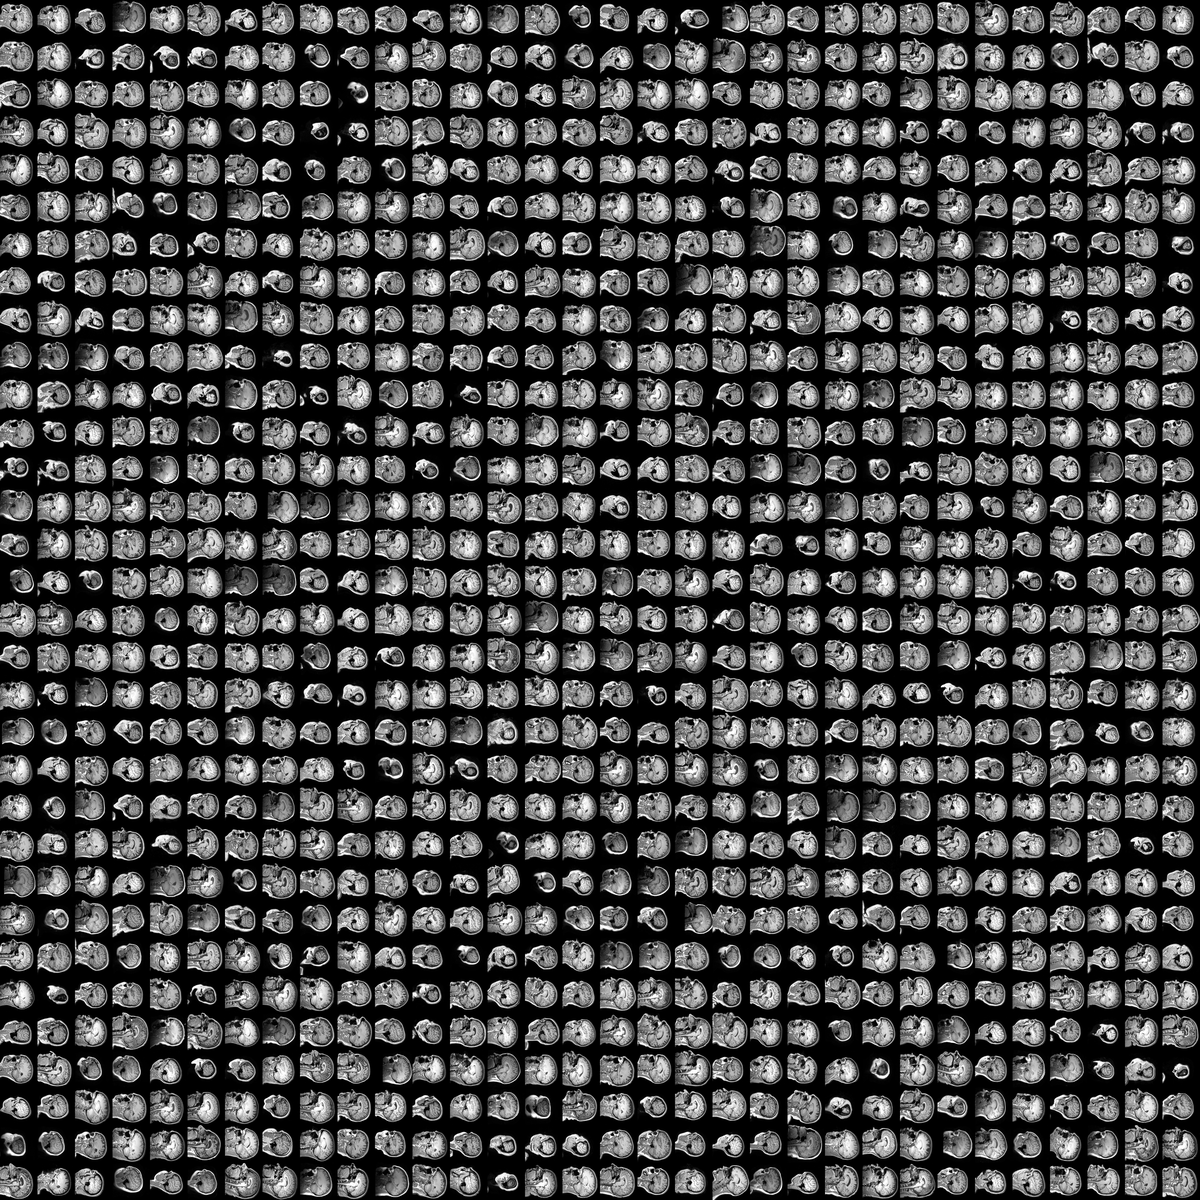
\includegraphics[width=0.82\textwidth]{figures/stylegan2_reals_preview.png}
\caption{StyleGAN2 训练集中真实 MRI 切片样本网格}
\label{fig:stylegan2-reals}
\end{figure}

训练完成后，项目得到可加载的模型快照 \texttt{network-snapshot-010000.pkl}。平台能够读取该权重并生成 MRI 切片，说明权重加载、潜变量采样、生成器推理、图像张量转换和 PNG 保存等环节已经连通。本文评价 StyleGAN2 结果时，重点不放在临床诊断性能上，而是关注生成链路可用性、输出可复现性和对三维输入的支撑能力。

\section{二维切片生成结果分析}
平台生成的示例切片如图 \ref{fig:generated-slices} 所示。该图来自生成切片结果目录，图像由训练完成的 StyleGAN2 权重生成。不同随机种子对应不同潜变量输入，系统由此得到不同灰度分布和结构形态的 MRI 切片示例。图中结果呈现出脑部 MRI 切片的基本轮廓和灰度结构，说明平台推理模块能够正确调用训练权重。

\begin{figure}[H]
\centering
\begin{subfigure}{0.32\textwidth}
\centering
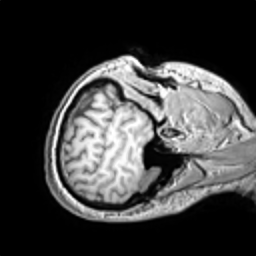
\includegraphics[width=\textwidth]{figures/generated_seed0123.png}
\caption{随机种子 123}
\end{subfigure}
\hspace{0.08\textwidth}
\begin{subfigure}{0.32\textwidth}
\centering
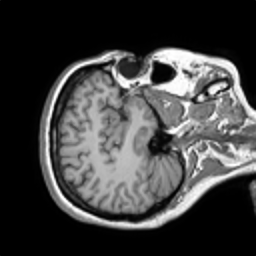
\includegraphics[width=\textwidth]{figures/generated_seed0042.png}
\caption{随机种子 42}
\end{subfigure}
\caption{StyleGAN2 生成的 MRI 切片示例}
\label{fig:generated-slices}
\end{figure}

二维切片生成链路已经形成闭环。用户在平台中指定模型权重、生成数量、截断参数和随机种子后，系统完成潜变量采样、生成器前向推理、灰度图像转换和结果保存。截断参数 \texttt{truncation\_psi} 用于调节生成结果的稳定性和多样性，随机种子则保证同一参数组合下结果可复现。该功能既可产生论文展示图，也可作为连续切片序列和点云初始化的输入。

\section{平台功能测试}
平台功能测试关注主要流程是否按预期运行。测试内容包括 FastAPI 后端接口、React 前端页面、数据预处理、模型训练入口、切片生成、连续序列生成、点云初始化、3DGS 结果展示和 AI 助手。测试结果显示，FastAPI 后端服务可以正常启动，React 前端可以访问平台页面；生成模块能够调用训练完成的权重输出 PNG 切片；点云初始化模块能够从切片目录生成 PLY 文件；3DGS 训练结果也能够以日志、渲染图像和点云文件形式归档。

\begin{table}[H]
\centering
\caption{平台主要功能测试结果}
\begin{tabular}{>{\raggedright\arraybackslash}p{3cm}>{\raggedright\arraybackslash}p{5.2cm}>{\raggedright\arraybackslash}p{4.8cm}}
\toprule
测试模块 & 测试内容 & 测试结果 \\
\midrule
数据预处理 & NIfTI 读取、轴向切片、归一化、缩放和 PNG 保存 & 已实现，可按数据目录批量处理 \\
模型训练 & 自动识别训练数据并启动 StyleGAN2 训练 & 已实现，训练结果已存在 \\
切片生成 & 加载 \texttt{.pkl} 权重并生成 PNG 图像 & 已通过，已有生成样例 \\
连续序列 & 潜空间插值得到连续切片序列 & 已实现，可用于三维展示 \\
点云初始化 & 将切片序列转换为 PLY 点云 & 已通过，已有 PLY 结果 \\
3DGS 重建 & 组织切片、点云、相机参数并完成训练输出 & 已通过，已有 checkpoint、点云和渲染结果 \\
FastAPI 后端 & 提供概览、生成、资产、任务、分析、报告和 AI 助手接口 & 已实现，可由 React 前端调用 \\
React 前端 & 提供仪表盘、生成、查看器、报告、可信性评估、任务、3D 和教学页面 & 已实现，可通过 Vite 本地服务访问 \\
AI 助手 & 参数说明和平台问答 & 已实现，包含本地解释逻辑和可选搜索接口 \\
\bottomrule
\end{tabular}
\end{table}

测试过程表明，平台已经具备毕业设计所需的演示能力。用户可以通过 React 前端完成从结果查看到二维生成，再到医学影像分析、可信性评估、三维表达和 3DGS 结果展示的主要流程。FastAPI 后端负责接口封装、任务状态和结果资产输出。平台首页、生成工作台、影像查看器、任务中心、点云展示页和异常提示共同构成系统展示材料。

\section{点云初始化结果分析}
点云初始化结果由 \texttt{init\_pcd.py} 生成，输出文件为 \texttt{init\_point\_cloud.ply}。该文件大小约 13 MB。PLY 文件头显示包含 477426 个顶点，每个顶点包含三维坐标和 RGB 颜色信息。点云预览如图 \ref{fig:init-point-cloud} 所示。

\begin{figure}[H]
\centering
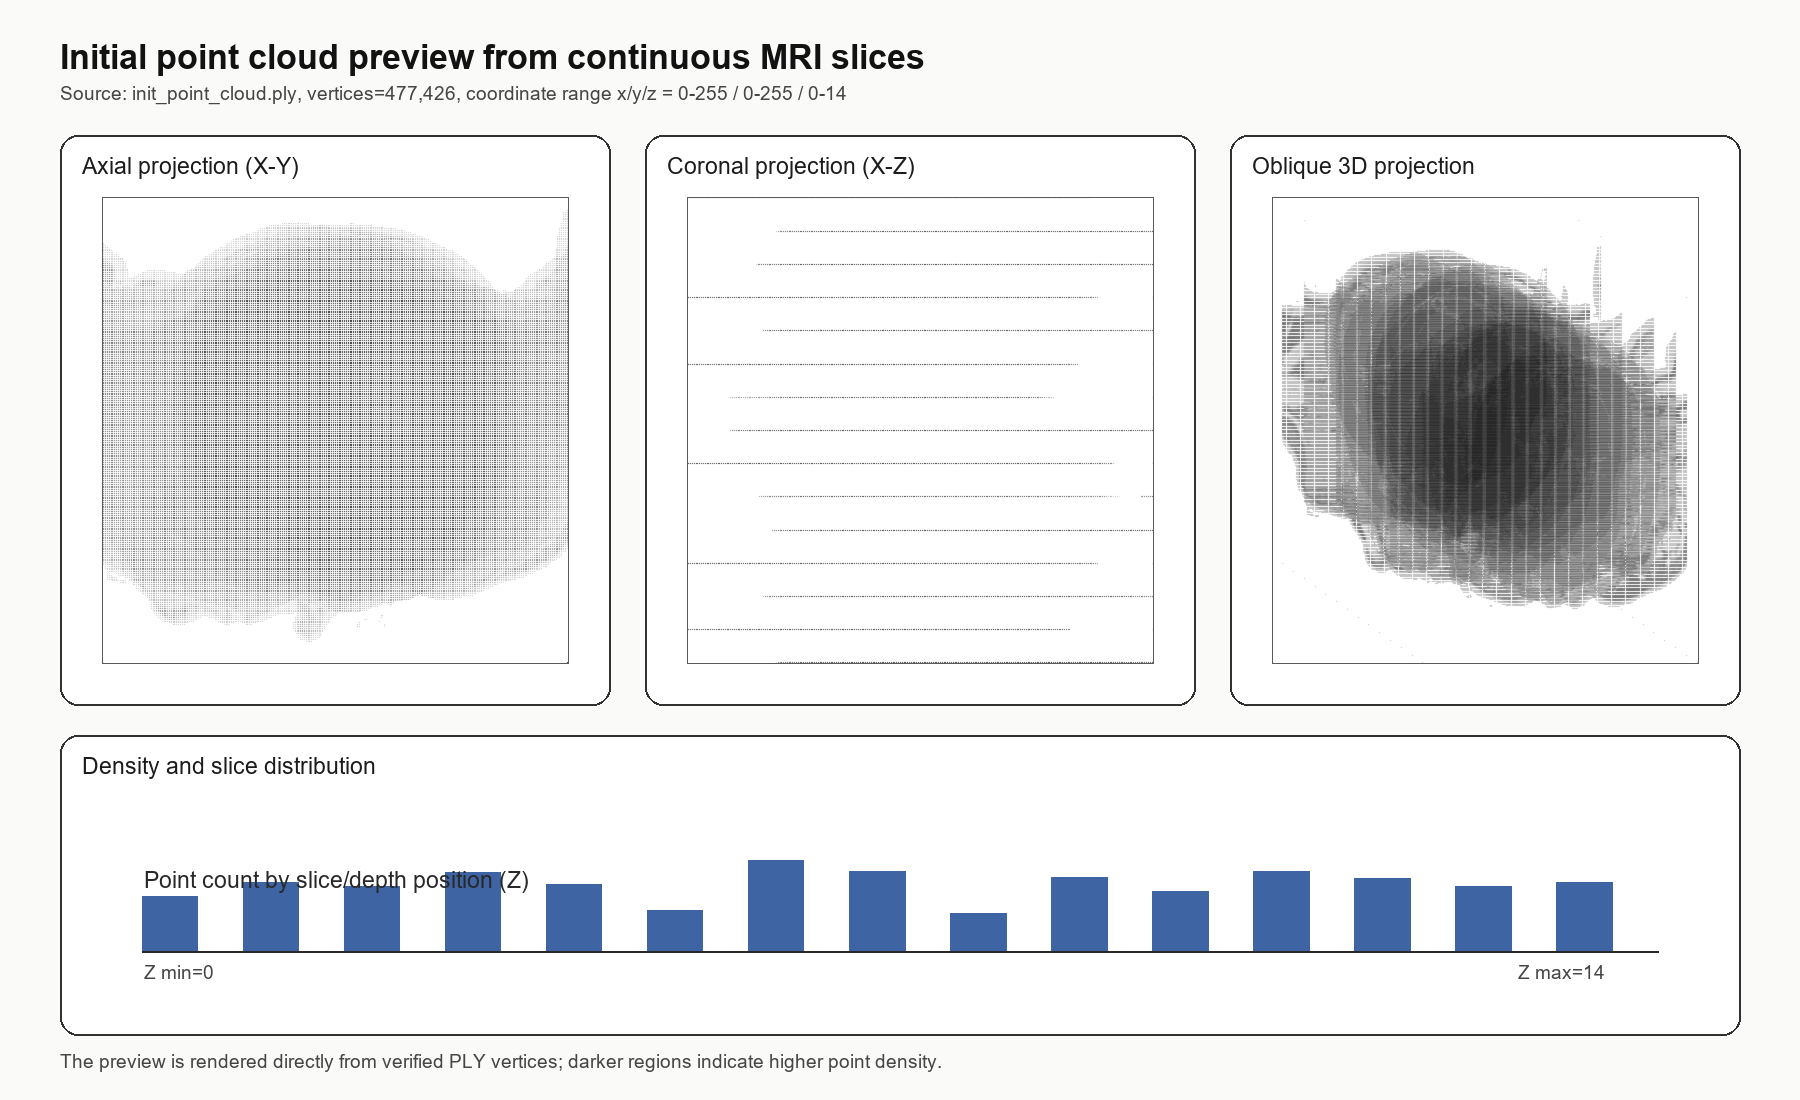
\includegraphics[width=0.82\textwidth]{figures/init_point_cloud_preview.png}
\caption{由连续 MRI 切片初始化得到的点云投影与密度分布预览}
\label{fig:init-point-cloud}
\end{figure}

该点云体现了二维切片进入三维空间的过程。每张切片对应一个 $z$ 轴位置，非背景像素对应空间点，像素灰度对应颜色强度。由此得到的点云既能作为 3DGS 三维重建输入，也能作为平台 2D/3D 对比展示的中间结果。与只展示单张二维图相比，该步骤提供了更明确的三维工程接口。

\section{3DGS 训练配置与重建结果}
3DGS 实验使用 180 张连续 MRI 切片作为监督图像，并以 300000 个点构建初始 PLY 点云。训练结果保存在 3DGS 主训练目录中。训练配置文件显示，模型采用三阶球谐函数表示颜色，输入图像目录为 \texttt{images}，数据设备为 CUDA。训练输出目录保存相机参数、checkpoint、训练日志、渲染结果和点云文件。

\begin{table}[H]
\centering
\caption{3DGS 训练主要参数与输出}
\begin{tabular}{>{\raggedright\arraybackslash}p{4.1cm}>{\raggedright\arraybackslash}p{8.2cm}}
\toprule
参数项 & 参数值或结果 \\
\midrule
训练切片数量 & 180 张 \\
训练图像分辨率 & $256\times256$ \\
初始点云规模 & 300000 点 \\
相机参数数量 & 180 个相机条目 \\
颜色表示 & 三阶球谐函数，\texttt{sh\_degree=3} \\
训练迭代次数 & 30000 轮 \\
最终 checkpoint & \texttt{chkpnt30000.pth} \\
最终点云 & 第 30000 轮输出 PLY 点云 \\
最终高斯点数量 & 572073 个 \\
\bottomrule
\end{tabular}
\end{table}

训练过程中，系统在第 1000、3000、5000、7000、15000 和 30000 轮记录训练集重建指标，也保存对应高斯点云。表 \ref{tab:3dgs-metrics} 给出了训练日志中的主要指标。随着迭代推进，L1 误差整体下降，PSNR 整体提高，说明三维高斯参数在切片监督下逐步逼近目标 MRI 切片分布。

\begin{table}[H]
\centering
\caption{3DGS 训练过程指标}
\label{tab:3dgs-metrics}
\begin{tabular}{cccc}
\toprule
迭代轮数 & L1 误差 & PSNR/dB & 说明 \\
\midrule
1000 & 0.1083 & 14.5942 & 初始优化阶段 \\
3000 & 0.0913 & 15.7418 & 结构逐步收敛 \\
5000 & 0.0881 & 15.8296 & 灰度细节增强 \\
7000 & 0.0873 & 15.8978 & 中期稳定优化 \\
15000 & 0.0806 & 16.4241 & 重建质量继续提升 \\
30000 & 0.0709 & 17.5894 & 最终训练结果 \\
\bottomrule
\end{tabular}
\end{table}

根据 180 对第 30000 轮渲染切片与参考切片计算，平均 PSNR 为 17.4738 dB，平均归一化 L1 为 0.0695，平均全局 SSIM 为 0.8935。这里的 SSIM 采用整幅灰度图全局统计方式计算，用于反映本平台实验中的重建一致性，而不是医学诊断性能指标。训练指标变化如图 \ref{fig:3dgs-metrics-30000} 所示。

\begin{figure}[H]
\centering
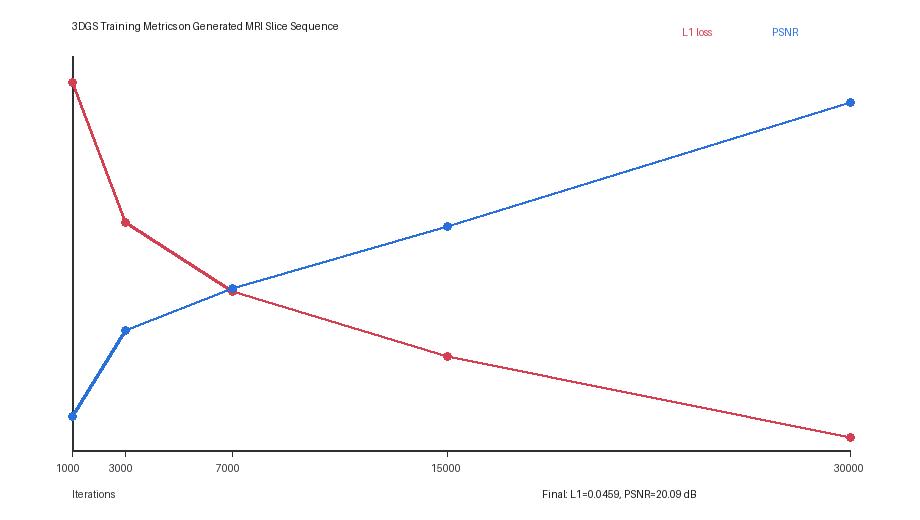
\includegraphics[width=0.9\textwidth]{figures/3dgs_metrics_30000.png}
\caption{3DGS 训练过程 L1 与 PSNR 指标变化}
\label{fig:3dgs-metrics-30000}
\end{figure}

第 30000 轮渲染切片与参考切片对比如图 \ref{fig:3dgs-comparison-30000} 所示。图中选取序列前部、中部和后部切片进行展示。渲染结果在脑部轮廓、主体灰度区域和层间变化趋势上与参考切片保持一致，但局部细节仍有一定平滑化现象。这与 MRI 灰度纹理、单序列输入约束和当前训练规模有关。

\begin{figure}[H]
\centering
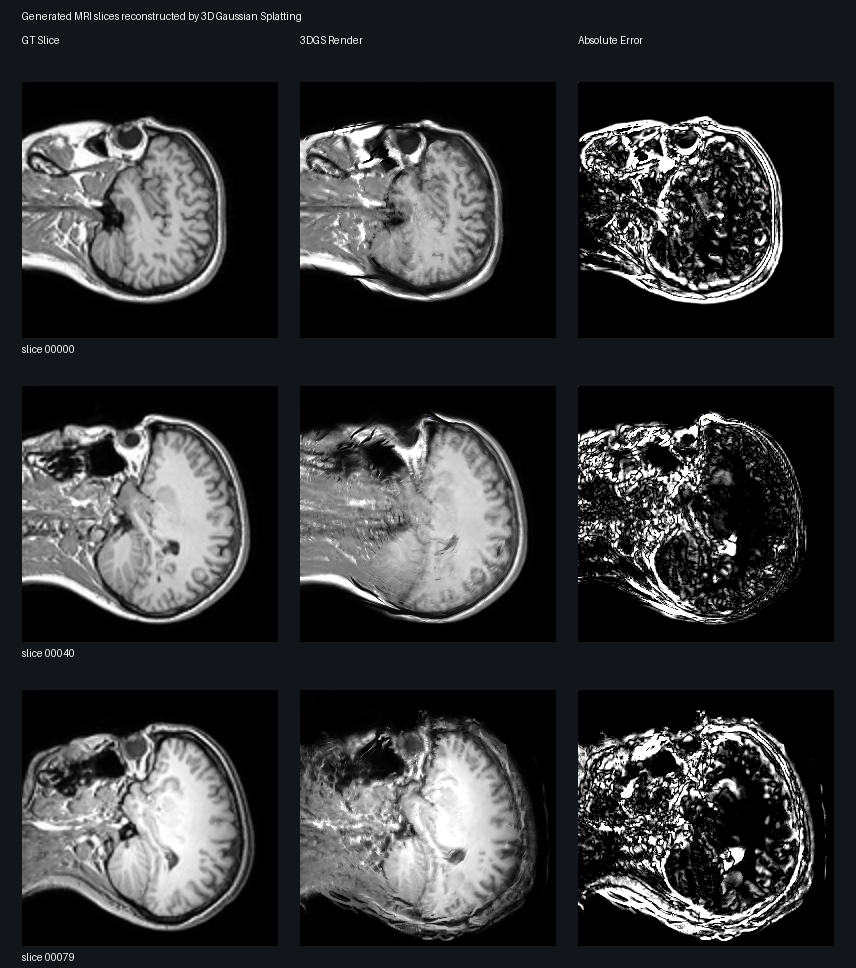
\includegraphics[width=0.82\textwidth]{figures/3dgs_slice_comparison_30000.png}
\caption{3DGS 第 30000 轮渲染切片与参考切片对比}
\label{fig:3dgs-comparison-30000}
\end{figure}

结合训练日志、checkpoint、点云文件和渲染结果可以确认，3DGS 模块已经完成训练闭环。该闭环从规则切片序列开始，并输出三维高斯表达。输入点云从 300000 点优化为 572073 个高斯点，说明训练过程在初始空间结构基础上调整并扩展了三维表达。该结果能够支撑平台开展 MRI 图像三维重建展示。

\section{综合评价与局限性分析}
本系统已经完成 MRI 数据预处理、StyleGAN2 二维生成、连续切片组织、点云初始化和 3DGS 三维重建的主要流程。StyleGAN2 部分形成了可加载权重和生成切片。3DGS 部分形成了训练日志、checkpoint、渲染图像和训练后点云。平台部分采用 FastAPI + React 架构，完成了后端接口、前端页面、任务状态、影像查看和三维展示。综合这些结果，系统满足毕业设计对算法实现、工程集成、实验验证和可视化展示的要求。

系统仍有提升空间。StyleGAN2 生成结果目前主要通过可视化和工程链路验证，后面可加入更大规模生成样本统计、专家评价或下游任务评价。3DGS 训练基于规则切片相机和单序列灰度图像，能够形成稳定的三维表达，但对细粒度组织边界的表达仍可继续改进。平台当前主要以本地 FastAPI 服务和 Vite 前端运行，后面可通过统一配置、环境变量和容器化方式提升跨环境部署能力。

\chapter{结论与展望}

\section{结论}
本文围绕“基于 3DGS 与 StyleGAN2 的 MRI 医学图像拟生成平台的设计与实现”开展研究，完成了从 MRI 数据预处理、二维切片生成、连续切片组织、点云初始化、3DGS 训练接入到前后端平台展示的整体设计与实现。论文工作不是单一算法复现，而是面向毕业设计场景，将医学图像数据处理、生成模型训练、三维表达和 Web 平台交互组织为一条可运行的工程链路。该链路能够支撑 MRI 切片生成、实验结果查看、三维资产展示和教学演示等任务。

本文的主要成果体现在四个方面。其一，系统实现了面向 NIfTI 格式 MRI 数据的预处理流程，包括切片提取、灰度归一化、尺寸调整、低质量切片过滤和训练数据整理，为后续模型训练提供了统一输入。其二，系统基于 StyleGAN2-ADA 完成二维 MRI 切片生成模型训练，并将训练权重接入平台推理流程，使用户能够通过随机种子和截断参数生成可复现的 MRI 切片结果。其三，系统将连续切片序列转换为 PLY 初始点云，并构建规则相机参数和训练输入，使 3DGS 能够用于 MRI 切片序列的三维表达实验。其四，系统采用 FastAPI 和 React 实现前后端分离平台，整合结果概览、切片生成、医学影像查看、任务管理、三维展示和 AI 助手等功能，提升了算法实验过程的可视化和可操作性。

本文的创新点主要体现在工程集成和医学图像生成流程适配上。第一，论文将 StyleGAN2 的二维切片生成能力与 3DGS 的三维高斯表达思路结合起来，形成“二维生成结果到三维表达”的平台化流程。第二，论文针对 MRI 切片序列具有规则层间关系这一特点，设计了由连续切片生成初始点云并组织 3DGS 输入的实现方法。第三，论文将训练、推理、结果管理和可视化统一到 FastAPI + React 平台中，使算法结果不再只停留在命令行和离线文件，而能够通过交互界面进行展示和分析。

实验与测试结果表明，平台具备较完整的教学演示和实验复现能力。StyleGAN2 训练链路已经形成可加载权重，平台能够基于该权重生成 MRI 切片。3DGS 部分能够在连续切片监督下完成训练，并输出三维高斯模型、渲染结果和训练指标。第 30000 轮训练达到 L1 为 0.0709、PSNR 为 17.5894 dB，180 对渲染切片与参考切片的平均全局 SSIM 为 0.8935。上述结果说明，本文构建的平台能够把二维生成、三维表达和结果展示连接起来，具有一定的工程应用价值和教学演示价值。

需要说明的是，StyleGAN2、StyleGAN2-ADA 和 3D Gaussian Splatting 的基础理论与核心模型来自已有公开研究，本文不将这些基础算法本身作为原创贡献。本文的本人研究工作主要集中在 MRI 数据处理流程设计、生成模型训练与推理接入、连续切片到点云和 3DGS 输入的工程适配、前后端平台实现，以及实验结果的整理与分析。这样的边界划分有助于明确本文贡献，也避免将已有科研成果误认为本文原创成果。

本研究仍存在一定局限。当前平台主要面向教学演示和工程验证，生成结果不能直接用于临床诊断。实验数据以脑部 T1 MRI 为主，数据类型和病例来源仍有限。3DGS 部分虽然能够完成训练和展示，但 MRI 切片序列不同于普通多视角照片，层间连续性、相机模型、空间尺度和医学结构一致性仍有改进空间。评价指标方面，本文已经使用 L1、PSNR、SSIM 和可视化对比进行分析，但还缺少医学专家评价和下游任务验证。

\section{展望}
后续研究可以从三维表达、评价体系、平台部署和应用场景四个方向继续推进。在三维表达方面，可以进一步结合 MRI 切片的真实层厚、体素间距和空间方向信息，改进相机参数构建方式，并加入层间连续性约束、结构平滑约束和高斯点裁剪策略，以提升边界细节和三维结构稳定性。对于 3DGS 与医学切片序列的结合，还可以探索更适合体数据的采样方式和渲染监督方式，使三维表达更加贴近医学图像本身的空间属性。

评价体系仍需要继续完善。后续可以在现有 L1、PSNR 和 SSIM 的基础上，引入 FID、LPIPS、分割一致性、病灶区域保持能力或下游任务性能等指标。对于医学图像生成任务，仅依靠视觉相似度并不足以说明结果可靠，因此还可以加入医学专业人员的主观评价和错误案例分析，从结构合理性、解剖一致性和教学可用性等角度评价生成结果。

平台工程也有进一步完善空间。当前系统已经能够通过本地 FastAPI 服务和 React 前端完成主要功能展示，但运行过程仍依赖本地模型路径、数据路径、GPU 环境和外部接口配置。后续可以通过配置文件、环境变量、任务队列和容器化部署方式规范运行环境，使平台更适合课程教学、实验复现和多人协作。对于耗时较长的训练任务，也可以加入更完善的日志追踪、失败恢复和资源监控功能。

应用场景方面，本文主要围绕脑部 T1 MRI 切片展开。后续可以扩展到多序列 MRI、CT 或其他公开医学图像数据集，也可以研究跨模态生成、数据增强和三维教学展示等任务。若未来能够获得更充分的数据、专家评价和伦理审查支持，平台还可以作为医学图像生成方法比较、三维重建流程教学和医学人工智能实验课程的辅助工具。


\cleardoublepage
\nocite{*}
\printbibliography[heading=bibintoc,title=参考文献]

\cleardoublepage
\chapter*{附\quad 录}
\thispagestyle{thesis-main}
\addcontentsline{toc}{chapter}{附录}
\markboth{成都信息工程大学学士学位论文}{成都信息工程大学学士学位论文}

如需加入附录内容，可在此处补充公式推导、补充图表、关键代码片段、实验记录或其他支撑材料。


\cleardoublepage
\chapter*{致\quad 谢}
\thispagestyle{thesis-main}
\addcontentsline{toc}{chapter}{致谢}
\markboth{成都信息工程大学学士学位论文}{成都信息工程大学学士学位论文}

在论文完成过程中，我得到了许多老师、同学和家人的帮助与支持。在此，谨向所有关心、指导和帮助过我的老师、同学及亲友表示诚挚的感谢。

首先，衷心感谢指导教师何长春讲师在选题确定、研究思路梳理、系统实现和论文撰写过程中给予的悉心指导与耐心帮助。其次，感谢人工智能学院各位老师在专业课程学习、科研训练和毕业设计过程中给予的支持，使我能够将生成式人工智能、医学图像处理和平台开发等知识应用到本课题中。最后，感谢家人和同学在学习与生活中的陪伴、鼓励与帮助。


\end{document}
